\documentclass{article}
\usepackage[a4paper]{geometry}
\usepackage[english]{babel}
\usepackage[utf8]{inputenc}
\usepackage{url}
\usepackage{hyperref}
\usepackage{graphicx}
\usepackage{amssymb}
\usepackage{amsmath}
\usepackage{amsfonts}
\usepackage{xspace}
\usepackage{yfonts}
\usepackage{mathrsfs}
\usepackage{amsthm}
\usepackage{graphicx}
\usepackage{algorithm}
\usepackage{algorithmicx}
\usepackage[noend]{algpseudocode}
\usepackage{multirow}
\usepackage{booktabs}
\usepackage{lscape}

\theoremstyle{definition}
\newtheorem{defn}{Definition}
\newtheorem{theorem}{Theorem}

\title{Project -  Multidimensional Unitary-profit Precedence-constrained Knapsack Problem}
\author{Lucas Guesser Targino da Silva - RA: 203534}

\newcommand{\nphard}{NP-hard\xspace}

\newcommand{\real}{\ensuremath{\mathbb{R}}\xspace}
\newcommand{\realnonnegative}{\ensuremath{\mathbb{R}_{+}}\xspace}
\newcommand{\realpositive}{\ensuremath{\mathbb{R}_{+}^{*}}\xspace}
\newcommand{\nrealnonnegative}[1]{\ensuremath{\mathbb{R}_{+}^{#1}}\xspace}
\newcommand{\nrealpositive}[1]{\ensuremath{\mathbb{R}_{+}^{*#1}}\xspace}

\newcommand{\true}{\ensuremath{true}\xspace}
\newcommand{\false}{\ensuremath{false}\xspace}

\newcommand{\subjectedTo}{\ensuremath{\mbox{subjected to}}\xspace}
\newcommand{\abs}[1]{\ensuremath{\left| #1 \right|}\xspace}
\newcommand{\tuple}[1]{#1-tuple\xspace}
\newcommand{\Set}[1]{\ensuremath{\left\{#1\right\}}}
\newcommand{\SetOf}[2]{\ensuremath{\left\{ #1 : #2 \right\}}\xspace}
\newcommand{\OrderedSet}[1]{\ensuremath{\langle#1\rangle}\xspace}
\newcommand{\function}[3]{\ensuremath{#1: #2 \rightarrow #3}\xspace}

\newcommand{\bigo}[1]{\ensuremath{\mathcal{O}\left( #1 \right)}}

\newcommand{\vehicleO}{\ensuremath{\upsilon}\xspace}
\newcommand{\vehicleSet}{\mathcal{V}\xspace}
\newcommand{\loadingFunction}{\ensuremath{\eta}\xspace}
\newcommand{\loadingFunctionApply}[1]{\loadingFunction \left( #1 \right)\xspace}
\newcommand{\loadingLimit}{\ensuremath{L}\xspace}
\newcommand{\nAxles}{\ensuremath{\alpha}\xspace}
\newcommand{\loadingCodomain}{\nrealnonnegative{\nAxles}}

\newcommand{\itemO}{\ensuremath{\iota}\xspace}
\newcommand{\itemSet}{\ensuremath{\mathcal{I}}\xspace}
\newcommand{\itemDomain}{\ensuremath{\nrealpositive{3} \times \nrealnonnegative{3}}\xspace}

\newcommand{\containero}{\ensuremath{c}\xspace}
\newcommand{\containerSet}{\ensuremath{\mathcal{C}}\xspace}

\newcommand{\lx}{\ensuremath{\chi}\xspace}
\newcommand{\ly}{\ensuremath{\psi}\xspace}
\newcommand{\lz}{\ensuremath{\omega}\xspace}
\newcommand{\px}{\ensuremath{x}\xspace}
\newcommand{\py}{\ensuremath{y}\xspace}
\newcommand{\pz}{\ensuremath{z}\xspace}

\newcommand{\itemInput}{\ensuremath{\mathit{I}_{o}}\xspace}
\newcommand{\itemOutput}{\ensuremath{\mathit{I}_{f}}\xspace}
\newcommand{\stackingPredicateSymbol}{\ensuremath{\mathcal{SC}}\xspace}
\newcommand{\stackingPredicate}[1]{\ensuremath{\stackingPredicateSymbol \left( #1 \right)}\xspace}

\newcommand{\vehicleInput}{\vehicleO}

\newcommand{\zoKPV}{0-1 Knapsack Problem\xspace}
\newcommand{\zoKP}{0-1KP\xspace}
\newcommand{\MKPV}{Multidimensional Knapsack Problem\xspace}
\newcommand{\MKP}{MKP\xspace}


\begin{document}

\maketitle

\begin{abstract}

We present a generalization of the classic 0-1 Knapsack Problem. In this problem, the weight of the items are multidimensional vectors and so is the knapsack capacity, the profit of all items is equal to one, and the items are required to be added in a certain order. That problem is refered as \textit{Multidimensional Unitary-profit Precedence-constrained Knapsack Problem (MEPKP)}. Three solution approaches are proposed: an Integer Linear Programming for a exact solution; a greedy algorithm for a fast solution; a Greedy Randomized Adaptive Search Procedures (GRASP) and Tabu Search (TS) for a near optimal solution. The three approaches will be compared in terms of quality of the solution and computational time with randomly generated instances.

\end{abstract}

\section{Problem Statement}

Given a graph $G = (V,E)$, with a multi-dimensional weight function $w: V \rightarrow \mathbb{R}_+^n$, where $n \in \mathbb N$, and a maximum capacity $W \in \mathbb{R}_+^n$.
Suppose that there is a partial order relation $\prec$ on $V$. We say that the tuple $(V,\prec)$ is partially ordered set. We'd like to remove the minimum amount of vertices in our graph such that, for every iteration, we remove a maximal element from our partially ordered set, so that $\sum\limits_{v \in S} w_v \leq W$ where $S \subseteq V$ is the set of remaining vertices at the end of our iterations.

The problem we propose here is a knapsack problem adapted to satisfy two extra constraints: partial ordering and multi-dimensional weights.


\section*{PLI Model}


\subsection*{Decision Variables}

\begin{equation}
    x_v :=  \begin{cases}
      1 & \mbox{Se $v \in V$ for retirado,} \\
      0 & \mbox{c.c.}
   \end{cases} \nonumber
\end{equation}

\setlength\parindent{72pt}
\subsection*{Linear Programming}

\begin{eqnarray}
    \label{constraint:stacking}
	\underset{S \subseteq V}{max} & \sum\limits_{v \in S} x_v \\
	s.t. & \nonumber\\
		 & \displaystyle\sum\limits_{v \in S} x_v w_v \leq W\\
		 & x_u \leq x_v  & \quad \forall (u,v) \in \prec \\
		 & x_v \in \{0,1\} & \quad \forall v \in V
\end{eqnarray}

\section{State of the Art}

In \cite{bib:grasp-and-tabu}, the authors proposes a memory based GRASP with restart and a simple tabu search algorithm is proposed to overcome the limitations of local optimality in order to find near optimal solutions. In that paper, numerical tests on benchmark instances demonstrate the effectiveness and efficiency of the proposed methodology which outperform the Mini-Swarm heuristic in terms of the success ratio, relative percentage deviation and computational time.

In \cite{bib:tabu-knapsack}, the authors reported the implementation of an efficient TS method based on the oscillation strategy and definition of a promising zone, a zone which englobes all factible solutions plus all infactible solutions bordering the infactible solutions, for solving the O-1 MKP which has been tested on standard test problems from \cite{bib:freville,bib:preprocessing-knapsack-1994} and \cite{bib:tabu-multidimensional-knapsack}. Optimal solutions were successfully obtained for all instances and the previously best known solutions were improved for five of the last seven instances. These numerical results were claimed to confirm the merit of tabu tunneling approaches to generate solutions of high quality for 0-1 multiknapsack problems. Moreover, these results (like those of \cite{bib:tabu-multidimensional-knapsack}) are claimed to establish that the oscillation strategy is efficient to balance the interaction between intensification and diversification strategies of TS.

In \cite{bib:constrained-knapsack}, the authors used a lagrangean relaxation on the precedence-constraint and the subgradient method to solve the problem faster then use a ``pegging'' test to guarantee optimality.


\subsection{0-1 Knapsack Problem}

\cite{bib:knapsack-problems} gives a definition for a \zoKPV (\zoKP):

\begin{eqnarray}
    \label{problem:knapsack-problem}
    \max & \displaystyle\sum\limits_{j=1}^{n} p_j x_j \\
    \subjectedTo
        & \displaystyle\sum\limits_{j=1}^{n} w_j x_j \leq c \nonumber\\
        & x_j \in \Set{0, 1} \quad \forall j \in \Set{1, \dots, n} \nonumber
\end{eqnarray}

in which $p_j$ and $w_j$ are know as the profit and the weight of the item $j$, respectively.

The problem proposed here is a knapsack problem adapted to satisfy two extra constraints: precedence-constrained and multi-dimensional weights. Besides, its profits are all one.

\section{Metaheurísticas}
\label{section:metaheuristics}

Nessa seção são descritas todas as metaheurísticas utilizadas ao longo do trabalho.

No desenvolvimento dos trabalhos anteriores, explorou-se variações de cada metaheurística, essas com diferentes parâmetros, estratégias construtivas, buscas locais, etc. Para cada metaheurística, foram selecionadas duas variações, as que apresentaram melhor desempenho, para serem utilizadas nas investigações deste trabalho.

\subsection{\greedyCriteriaText}

Since the problem is a unitary-profit, the objective function provides no information about which vertex is better to add to the solution. Being more practical, for designing an algorithm, making decisions based solely on the objective function is useless and meaningless. For that reason, we propose the following auxiliary function $\greedy$, called \greedyCriteriaText:

\begin{defn}[\greedyCriteriaText]
    \label{def:greedy-criteria}
    Let  be a vertex and $\weightE$ its weight. The \greedyCriteriaText is the function $\function{\greedy}{\vertices}{\positiveInteger}$ which associates a vertex $\solutionE \in \vertices$ to the entry of its weight vector $\weightE \in \weightCodomain$ with the highest value:
    \begin{equation}
        \label{eq:greedy-criteria}
        \apply{\greedy}{\solutionE} = \apply{\max}{\weightE}
    \end{equation}
\end{defn}

In metaheuristics, we are usually interested in greedy strategies. For the approaches analyzed in this project, the greedy criteria is going to be: select the vertex which minimizes the value of $\greedy$. The intuition behind such choice is clear: we want to add vertices which weight as little as possible.

Notice that the above definition is not the only one available. One could choose to use the norm 2 or average value of the weight vector $\weightE$. The election of the maximum is relies on the intuition that ``averages'' might fill too much one of the dimensions of the weight while leaving others free. That would cause early stop of the algorithms. The maximum function, on the other hand, ensures that dominating values of the dimension of the weight are properly handled.

Of course, using the maximum function has drawbacks as well. Since it looks only to the most loaded entry, between two vertices with the same value of the greedy function $\greedy$, it won't see which one has lower values in the other entries.

\section{Integer Linear Programming Model}

\subsection{Decision Variables}

\begin{equation}
    \label{eq:decision-variables}
    \varE =  \begin{cases}
      1 &, \solutionE \in \solution \\
      0 &, \solutionE \notin \solution
   \end{cases}
\end{equation}

\subsection{Mathematical Model}

\begin{align}
    \label{eq:ILP-objective}
    \max\limits_{\solution \subseteq \vertices}
        & \Sum{\solutionE \in \solution}{}{\varE} \\
    s.t.
    \label{eq:ILP-capacity-constraint}
    & \Sum{\solutionE \in \solution}{}{\varE \weightE} \leqslant \maximumWeight \\
    \label{eq:ILP-order-constraint}
    & \var_{\solutionE} \leqslant \var_{\solutionEp} \quad \forall \solutionEp \partialLower \solutionE \\
    \label{eq:ILP-binary-constraint}
    & \var \in \varDomain
\end{align}

\eqref{eq:ILP-objective} is the objective function: maximize the number of vertices in the solution.
\eqref{eq:ILP-capacity-constraint} is the Capacity-Constraint of \eqref{eq:capacity-constraint}.
\eqref{eq:ILP-order-constraint} is the Precedence-Constraint of \eqref{eq:precedence-constraint}: if a vertex $\solutionE$ is in the solution, then all vertices $\solutionEp$ for which there is a path from $\solutionE$ must also be in the solution.

\subsection{GRASP + Tabu Search}

In order to find a time optimal algorithm to solve \MUPKP, we propose a comparative analysis of an implementation of a Integer Linear Program to solve MPKP and a near optimal algorithm utilizing GRASP and Tabu Search as GRASP's local search.

\begin{algorithm}[ht!]
    \caption{GRASP Pseudocode}
    \begin{algorithmic}[1]
        \Require{$MaxIterations, Seed$}
        \For{$k=1,\ldots,MaxIterations$}
            \State{$Solution \leftarrow Greedy Randomized Construction(Seed);$}
            \If{Solution is not feasible}
                \State{$Solution \leftarrow Repair(Solution)$;}
            \EndIf
            \State{$Solution \leftarrow LocalSearch(Solution);$}
            \State{$UpdateSolution(Solution, BestSolution);$}
        \EndFor
        \\\Return{$BestSolution$}
    \end{algorithmic}
\end{algorithm}
where the candidate list is build greedily utilizing the current maximal elements on our input graph(as long as they fit).
There's no need to use any repair method as the solution built from the candidate list will always fit in the knapsack.
That way, we do a local search and update our solution with the best one seen to far.

The trick here is to use a Tabu Search, instead of a naive local search method, to both avoid falling in local optima and utilizing the tabu list in order to avoid repeating moves and other. We use GRASP as a diversification strategy.

We now define exactly how this search is proposed.

Let $n \in \mathbb N$ be the number of binary variables of an input instance. The tabu list, let's call it $Tabu$ is a mapping $Tabu : StrN \rightarrow \mathbb N$, with pre-defined $Tabu.size$ capacity, where $StrN$ is an arrangement of $n$ bits let's call it $Arr$, where $n$ is the number of binary variables of our instance, and the $i$-th bit represents the state of $x_i$, where $Arr[i] = x_i$.

We also utilize a heap structure to get the earliest added tabu in $O(1)$ time.

During the local search, at each iteration we add the current state of our binary variables an element of $Tabu$. If the total number of tabus is equal to $Tabu.size$ we pop the earliest added tabu from our heap and remove that tabu from $Tabu$ while adding the new move to $Tabu$.

Each time that the Tabu Search tries to do a tabu move the integer in $Tabu$ associated with this move is looked up by the search, if the tabu exists, and if it equals $1$, that tabu is removed from the mapping.

Each move in the Tabu Search is a bit flip operation of a variable in a randomly selected, at every search iteration, subset $BinVars$ of the set of all binary variables of the input instance, such that $|BinVars| = k <= n$, where $k \in \mathbb{N}$ is a pre-defined parameter, as a way to limit the search space of the Tabu Search.

The best values for $k$ and $Tabu.size$ will be determined by tests.

\subsection{Greedy Algorithm}

It is a simple algorithm: add the vertices which minimize the added weight and does not violate the precedence-constraint iteratively until no more vertex can be added without exceeding the knapsack capacity. Such algorithm is presented below:

\begin{algorithm}[ht!]
    \caption{Greedy}
    \begin{algorithmic}[1]
        \Require{$\vertices, \edges, \weight, \maximumWeight$}
        \State{$S \gets \emptyset$}
        \State{$X \gets $ all leaf vertices}
        \State{$Y \gets 0$}
        \State{$\solutionE \gets \mathop{\mathrm{arg\,min}}\limits_{\solutionE \in X} \weightE$}
        \While{$Y + \weightE \leqslant \maximumWeight$}
            \State{$S \gets S \cup \Set{\solutionE}$}
            \State{$Y \gets Y + \weightE$}
            \State{$X \gets $ all the vertices not yet in $S$ that can be added to $S$ without violating the constraints}
            \State{$\solutionE \gets \mathop{\mathrm{arg\,min}}\limits_{\solutionE \in X} \norm{\weightE}$}
        \EndWhile
        \\\Return{$S$}
    \end{algorithmic}
    \label{algorithm:greedy}
\end{algorithm}


\section{Instance Generation}

The instances are generated randomly \cite{bib:instances-CVRP}, \cite{bib:constrained-knapsack}, \cite{bib:grasp-and-tabu}. For that, first the graph is generated, and then the weight of each vertex is chosen. The knapsack capacity is selected so that, on average, X percent of the vertices fit in it. The following subsections analyze each of those aspects.

Consider the parameters:
\begin{enumerate}
    \item $n$: number of vertices;
    \item $K$: average number of branches;
    \item $L$: maximum number of leaf vertices;
    \item $H$: the maximum value of an entry of the weight of each vertex;
    \item $m$: fraction of the average number of elements that fit in the knapsack;
\end{enumerate}

\subsection{How to Generate the Precedences}

The process of generating the precedences is specified in \algref{algorith:find-trees}, which uses \algref{algorith:generate-precedences}. The \figref{fig:precedence-generation} has an example of such procedure. The following parameters are used to control the generation:

\begin{algorithm}
    \caption{Find-Trees}
    \label{algorith:find-trees}
    \begin{algorithmic}[1]
        \Require{
            $\vertices$: vertices in the 2D plane,
            $K$: average number of branches,
            $L$: maximum number of leaf vertices
        }
        \State{$k \gets $ random number from 1 to $K$}
        \State{$\tuple{R, \mathcal{V}} \gets $ find $k$ clusters in $V$}
            \Comment{$R$: a set of centers}\\
            \Comment{$\mathcal{V}$: a set with each element being the set vertices of each cluster}
        \State{$\mathcal{T} \gets \emptyset$}
        \For{each pair $r \in R $ and $V' \in \mathcal{V}$}
            \If{$\abs{V'} \leqslant L$}
                \State{$T \gets $ tree with $r$ as the root node and $V'$ as the leaves}
            \Else
                \State{$T \gets $ tree with $r$ as the root node of the subtree Find-Trees($V', K, L$)}
            \EndIf
            \State{$\mathcal{T} \gets \mathcal{T} \cup \Set{T}$}
        \EndFor
        \\\Return{$\mathcal{T}$}
    \end{algorithmic}
\end{algorithm}

\begin{algorithm}
    \caption{Generate-Precedences}
    \label{algorith:generate-precedences}
    \begin{algorithmic}[1]
        \Require{
            $n$: number of vertices,
            $K$: average number of branches,
            $L$: maximum number of leaf vertices
        }
        \State{$V \gets $ generate $n$ points in the 2D plane randomly}
        \State{$\mathcal{T} \gets $ Find-Trees($V, K, L$)}
        \\\Return{$\mathcal{T}$}
    \end{algorithmic}
\end{algorithm}

\begin{figure}[ht!]
    \centering
    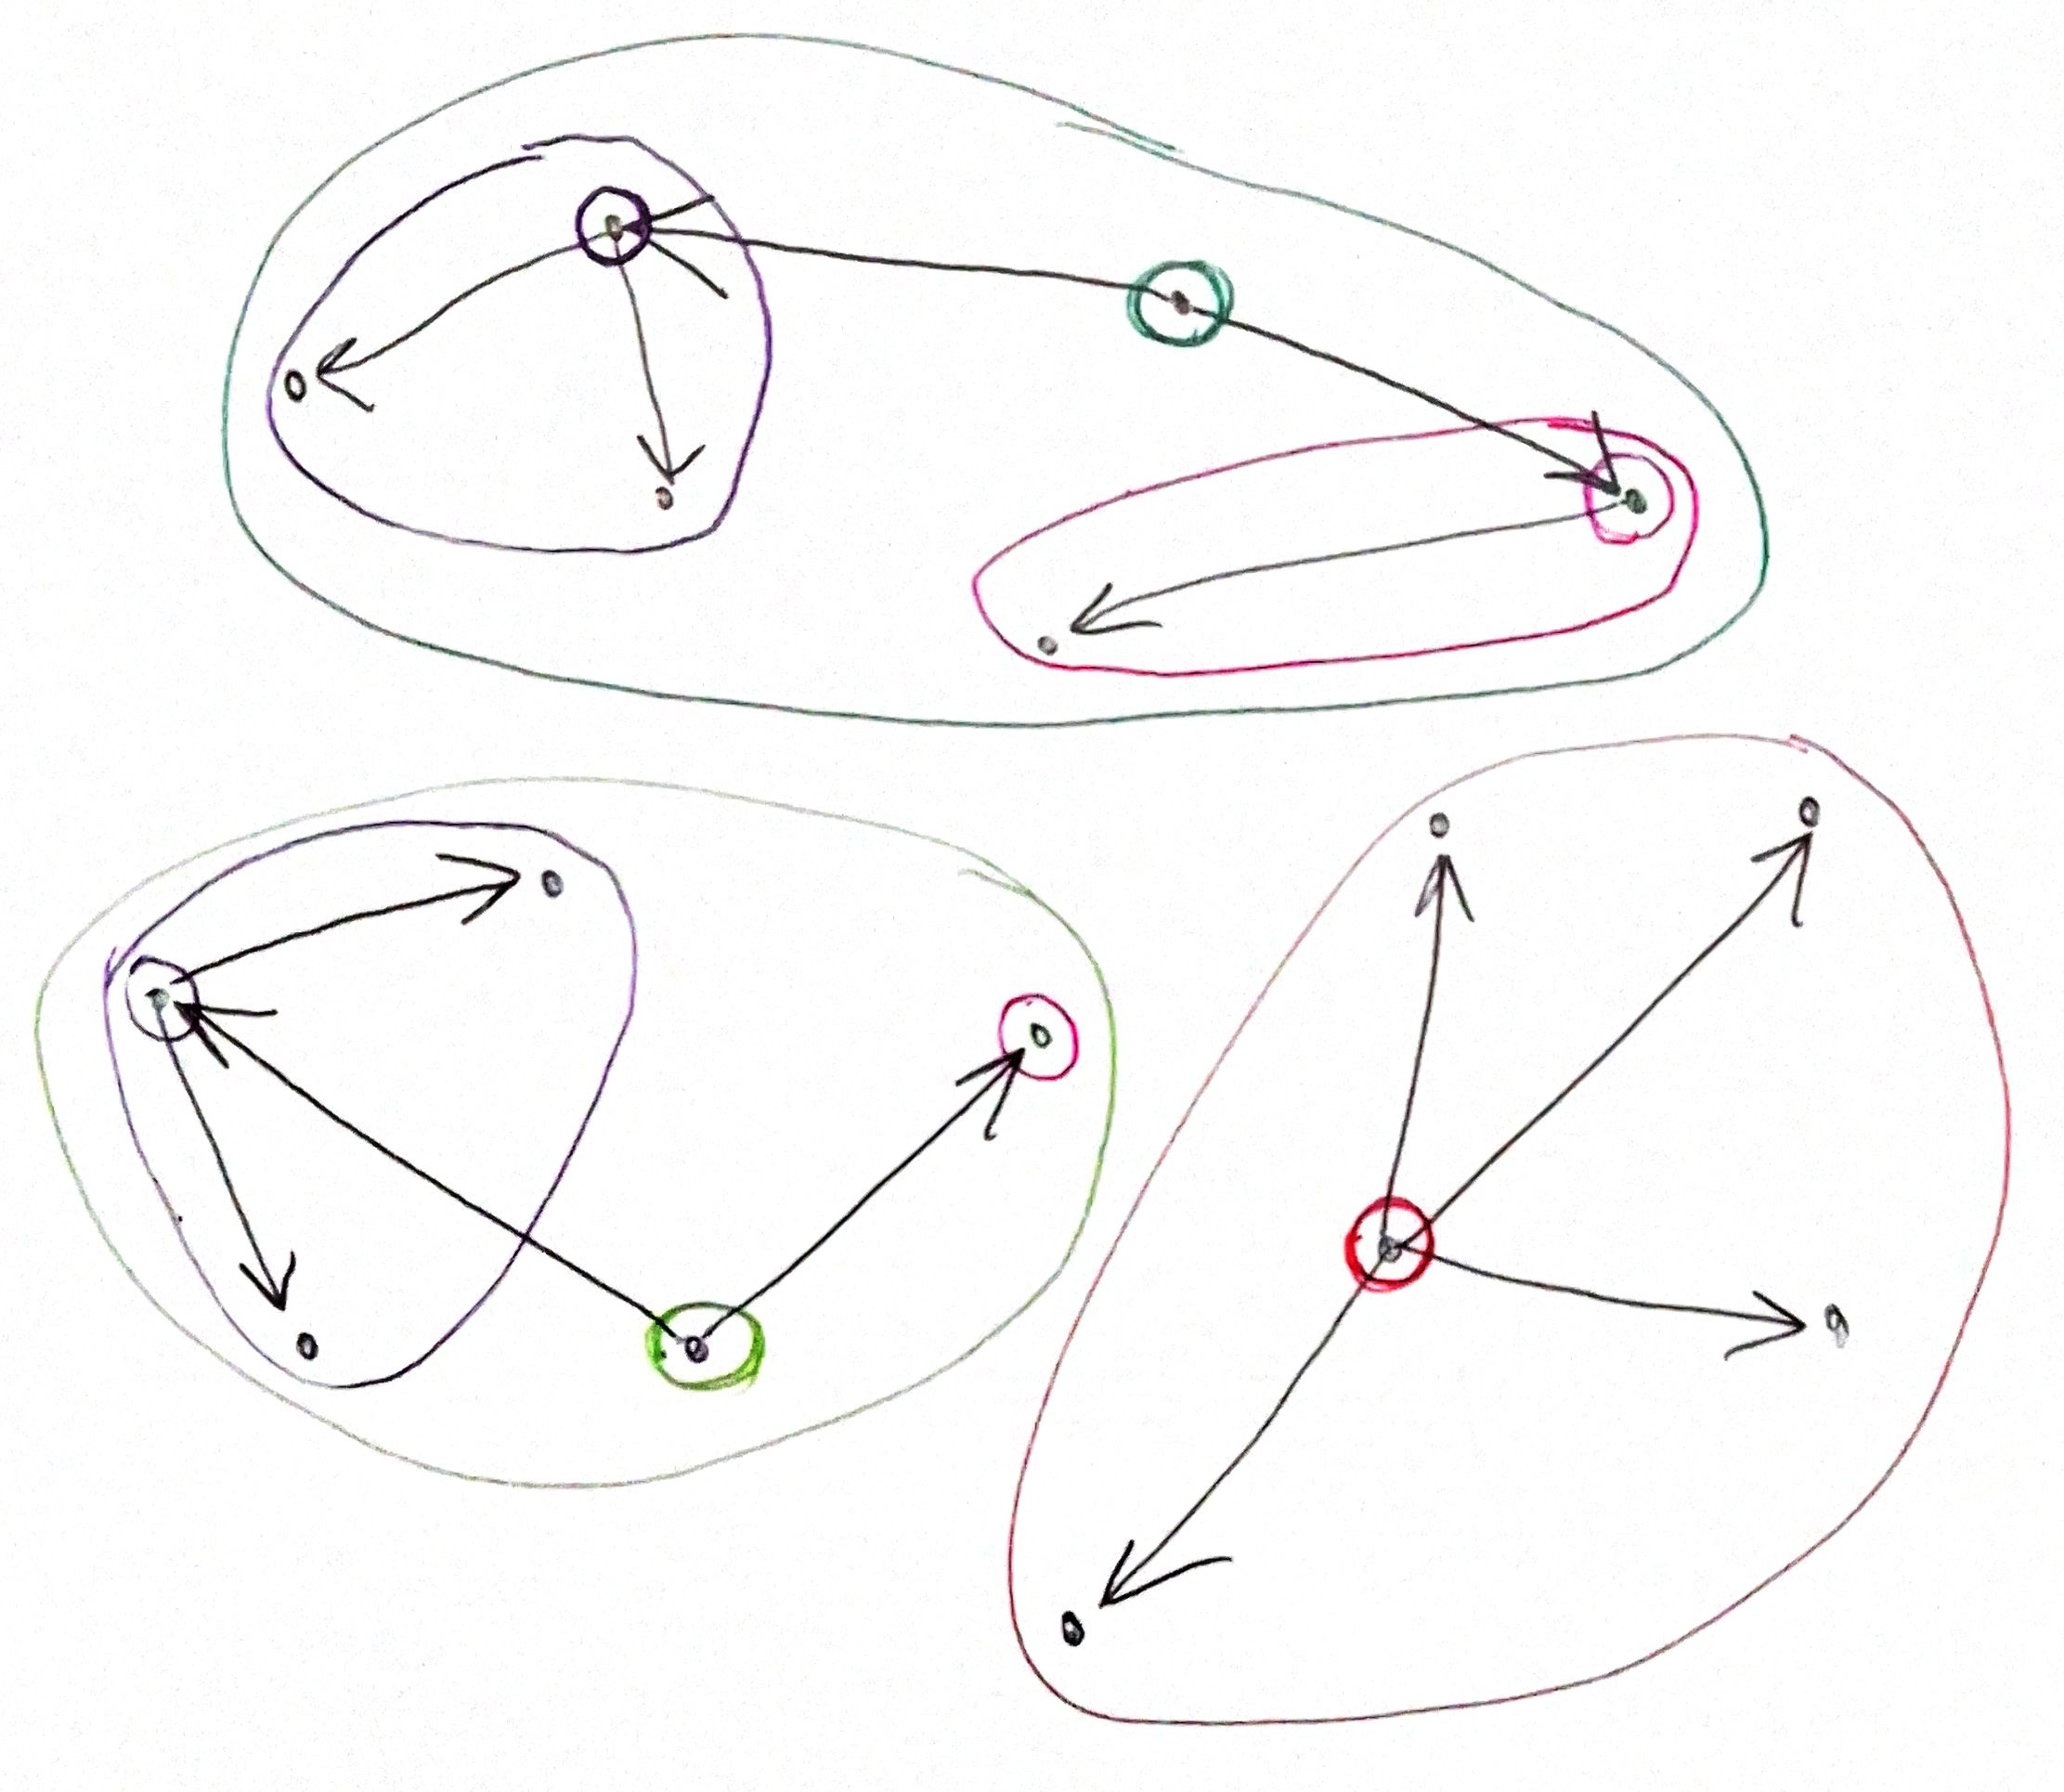
\includegraphics[width=0.5\textwidth]{images/precedence_construction.jpg}
    \caption{Precedence generation. The root nodes are the green, red and lemon. Red has four leaf vertices. Green has two branches, the pink with one leaf and the purple with two leaves. Lemon has one leaf and one branch with two leaves.}
    \label{fig:precedence-generation}
\end{figure}

\subsection{How to Generate the Weights}

Generate the weights randomly in the interval $\interval{0}{H}$.

\subsection{How to Generate the Knapsack Capacity}

Generate each entry of the knapsack capacity $\maximumWeight$ randomly in the interval $\interval{0}{m \cdot n \cdot H}$.

\section{How to evaluate the Results}

We will generate a table with the result of the experiments in the format below. Graphics are going to be created on demand as we analyze the results. Such results will provide all the information required to see how each method behaves, how different instances impact on each method, how big is the instance they can handle.

\begin{table}[ht!]
    \centering
    \begin{tabular}{|c|c|c|c|c|c|c|}
        \hline
        \multirow{2}{*}{Instance} &
            \multicolumn{2}{c|}{ILP} &
            \multicolumn{2}{c|}{greedy} &
            \multicolumn{2}{c|}{metaheuristic} \\
            & no. items & time & no. items & time & no. items & time\\
        \hline\hline
        X & 10 & 100 & 8 & 14 & 9 & 36 \\
        \hline
    \end{tabular}
    \caption{Results of the methods of solution. The time is given in seconds.}
\end{table}


\section{Results}

\begin{landscape}

\begin{table}
\centering
\begin{tabular}{lrrrrrrrrrrr}
\toprule
name & \multicolumn{3}{l}{problem\_info} & \multicolumn{2}{l}{ilp} & \multicolumn{2}{l}{greedy} & \multicolumn{2}{l}{grasp} & \multicolumn{2}{l}{tabu} \\
{} &     capacity & edges & nodes & cost &   time[s] &   cost & time[s] &  cost & time[s] & cost & time[s] \\
problem          &              &       &       &      &           &        &         &       &         &      &         \\
\midrule
N100\_E0\_W51666   &        51666 &     0 &   100 &   72 &  0.001373 &     69 &   0.008 &    70 &   0.031 &   70 &   0.025 \\
N100\_E0\_W52398   &        52398 &     0 &   100 &   72 &  0.002125 &     69 &   0.039 &    69 &   0.126 &   69 &   0.102 \\
N100\_E111\_W52365 &        52365 &   111 &   100 &   71 &  0.002847 &     70 &   0.009 &    70 &   0.025 &   70 &   0.044 \\
N100\_E118\_W52247 &        52247 &   118 &   100 &   71 &  0.003379 &     70 &   0.017 &    71 &   0.043 &   70 &   0.078 \\
N100\_E213\_W52199 &        52199 &   213 &   100 &   70 &  0.006474 &     70 &   0.006 &    70 &   0.014 &   69 &   0.056 \\
N100\_E222\_W53297 &        53297 &   222 &   100 &   70 &  0.011230 &     69 &   0.002 &    69 &   0.014 &   69 &   0.036 \\
\bottomrule
\end{tabular}
\caption{Cost and running time of all metaheuristics for problem instances with 100 nodes.}
\label{table:100-results}
\end{table}

\end{landscape}

\begin{landscape}

\begin{table}
\centering
\begin{tabular}{lrrrrrrrrrrr}
\toprule
name & \multicolumn{3}{l}{problem\_info} & \multicolumn{2}{l}{ilp} & \multicolumn{2}{l}{greedy} & \multicolumn{2}{l}{grasp} & \multicolumn{2}{l}{tabu} \\
{} &     capacity & edges & nodes & cost &   time[s] &   cost & time[s] &  cost & time[s] & cost & time[s] \\
problem            &              &       &       &      &           &        &         &       &         &      &         \\
\midrule
N500\_E570\_W262641  &       262641 &   570 &   500 &  361 &  0.010798 &    355 &   0.129 &   355 &   1.729 &  353 &   1.086 \\
N500\_E594\_W262931  &       262931 &   594 &   500 &  360 &  0.017267 &    353 &   0.127 &   356 &   1.524 &  353 &   1.040 \\
N500\_E598\_W263031  &       263031 &   598 &   500 &  359 &  0.024541 &    353 &   0.245 &   354 &   1.985 &  353 &   1.712 \\
N500\_E1157\_W262412 &       262412 &  1157 &   500 &  357 &  0.065347 &    351 &   0.072 &   353 &   0.595 &  352 &   1.046 \\
N500\_E1169\_W262155 &       262155 &  1169 &   500 &  356 &  0.061799 &    350 &   0.036 &   353 &   0.583 &  351 &   1.016 \\
N500\_E1189\_W260774 &       260774 &  1189 &   500 &  357 &  0.056502 &    353 &   0.058 &   353 &   0.621 &  351 &   0.990 \\
\bottomrule
\end{tabular}
\caption{Cost and running time of all metaheuristics for problem instances with 500 nodes.}
\label{table:500-results}
\end{table}

\end{landscape}

\begin{landscape}

\begin{table}
\centering
\begin{tabular}{lrrrrrrrrr}
\toprule
name & \multicolumn{3}{l}{problem\_info} & \multicolumn{2}{l}{greedy} & \multicolumn{2}{l}{grasp} & \multicolumn{2}{l}{tabu} \\
{} &     capacity & edges & nodes &   cost & time[s] &  cost & time[s] & cost & time[s] \\
problem             &              &       &       &        &         &       &         &      &         \\
\midrule
N1000\_E954\_W523944  &       523944 &   954 &  1000 &    707 &   1.311 &   710 &  27.659 &  707 &   8.613 \\
N1000\_E975\_W523980  &       523980 &   975 &  1000 &    708 &   0.702 &   712 &  22.837 &  712 &   7.913 \\
N1000\_E1017\_W523215 &       523215 &  1017 &  1000 &    708 &   0.751 &   711 &  22.985 &  708 &   8.659 \\
N1000\_E1925\_W523221 &       523221 &  1925 &  1000 &    706 &   0.489 &   707 &  10.759 &  703 &   7.565 \\
N1000\_E1956\_W527027 &       527027 &  1956 &  1000 &    705 &   0.549 &   708 &  10.030 &  705 &   7.726 \\
N1000\_E2032\_W526397 &       526397 &  2032 &  1000 &    706 &   0.235 &   708 &   7.158 &  701 &   6.929 \\
\bottomrule
\end{tabular}
\caption{Cost and running time of all metaheuristics for problem instances with 1000 nodes.}
\label{table:1000-results}
\end{table}

\end{landscape}



\bibliographystyle{unsrt}
\bibliography{bibliography}


\end{document}
